%# -*- coding: utf-8-unix -*-
%%==================================================
\chapter{项目解析}
\label{chap1}
\begin{itemize}[noitemsep,topsep=0pt,parsep=0pt,partopsep=0pt]
	\item ...
\end{itemize}

\section{知识点和方法论}
\subsubsection{华为软件精英挑战赛2020}
2020年华为软挑是对金融风控的查询, 简单来说实现了一个对于循环转账3-7个账号循环转账的监测. 对于算法时间的优化. \par
刚开始使用string字符串, 结果因为string字符串基于堆, 生成和释放比较消耗时间, 我们使用了全局静态变量, 用来简化字符串的生成. 以空间换时间. 后来经过测试没有自己写的char数组转int快, 后来换成自己写的转换函数了 \par
使用mmap进行内存映射, 减少IO读取时间(普通的read会拷贝一次到内核缓冲区). 再将整个缓冲区用fwrite写入文件,因为fwrite带有缓冲区, 比write而言, write使用的是系统缓冲区, 可能会增加IO次数.\par
使用dfs然后最开始使用了7层dfs+回溯. 十分耗时, 然后, 我实现了6+1层dfs, 减少了一层dfs. 减少一层是通过开始节点的入度判定的, 遍历6层之后, 如果下一个节点是头结点的. 那么结束循环保存答案\par
后来进一步优化, 使用 5+2(反向) dfs 减少时间. 先反向遍历两层, 然后再正向遍历5层, 当遍历到第5层的时候, 如果是两次反向遍历可以达到head节点, 的话, 我们就输出答案. \par
进一步优化, 使用反向遍历3进行剪枝, 如果访问超过了3层, 但是反向遍历3层不是头结点, 那么进行剪枝 \par
均匀使用四个区间, 开启四个线程进行运算 \par
\subsubsection{华为软件精英挑战赛2021}
华为软挑是实现云计算背景下的服务器资源分配和调度问题.  核心构成就是策略的使用, 使金额最小 \par
给定一些服务器与虚拟机,每日会有一定量的创建与删除虚拟机请求,我们需要合理安排服务器的购买和虚拟机请求的分配,从而达到购买服务器的成本和能耗成本的总和最低。一台服务器的抽象化为两个CPU分区, 和 两个内存分区.  虚拟机也抽象化为可以单部署 和双部署, 双部署就是, 对于一台服务器而言 要均衡的放在两个CPU分区, 和两个内存分区. \par
团队是qq群中组建的, 一个浙大的研究生, 两个杭电的研究生. 因为杭电和浙大还是距离挺远的, 我们采用了线上开会的形式.  代码采用了github的方式进行同步. 简单讲一下我们的校验手段, 比赛开始之后一段时间, github上就有了可视化平台, 我们利用可视化平台可以比较详细的看出, 我们购买的服务器的种类, 和购买的个数.  还有整个系统的波动曲线, 就是购买个数之类的. 每日能耗曲线之类的. \par
这个问题我们探讨出有两个点可以进行集中优化. \par

A. 即购买策略\par
a. 将当天需要购买的虚拟机按照, CPU数量和内存数量的和进行排序, 降序排序\par
b. 然后寻找一个服务器开着的, 然后尝试将虚拟机放入服务器, 选择服务器的使用率最高的那个, 进行存放.\par
c. 如果没有成功放置进入C环节, 选择一台关机了的服务器, 进行存放.\par
d. 还没成功选择, 选择一台服务器 刚开始我们使用的是, 恰恰能放入虚拟机的服务器. 后期我们进行了更新, 选择,能放入这台服务器和前面已经存放的服务器的大小, 就是留有一定的余量. 可以减少购买服务器的资金.\par
B. 迁移的策略\par
a. 我们每天可以进行一次服务器迁移, 这样将利用率低的服务器从低到高进行排序, 然后将利用率低的服务器迁移到利用率高的服务器.\par
b. 后期我们增加了一个简单的策略. 将一台服务器中只有一个和两个的挑选出来, 放入其他的服务器中, 这样可以带来省电的效果.\par

前期我们首先三个人每个人按照自己的想法制作了一个基线版本, 为什么要写一个基线版本呢? 这样我们对整个问题都有一个比较深刻的认识, 后期, 我们更具我们建模出来的可以比较提升系统性能的地方, 进行了改进.
对于 购买策略, 和迁移策略进行改进. 我个人对于购买策略和系统参数进行了调试. 购买策略的排序和余量设定, 给我的系统带来了大约2000w的资金节省.调试参数, 就是在题目要求的时间边缘进行反复测试直到达到一个最优值, 前期 我们设定的参数是低于30\% 的利用率我们会进行迁移, 这样迁移的机器数量比较少, 并不能达到我们的预期, 后期我进行慢慢测试终于选定了50\%这个参数, 选了更大的参数大部分服务器都要进行迁移, 反而效果并不是特别好. \par
迁移策略由另外两个同学进行改进. 迁移策略我印象比较深刻的地方是, 因为排行榜上前几名的系统迁移基本上拉满了, 我们还有很多的余量. 所以他们连个进行了这个开发.
他们使用了类似于快速排序点的方法进行迁移. 按照服务器日常能耗的价格进行排序, 然后设定两个指针, 一个指针指向价格比较低的地方, 一个指针指向价格高的地方,然后尝试将价格高的服务器迁移到价格低的服务器上, 如果成功, 然后右指针--, 如果失败左指针++. 直到两个指针相遇. 但是因为比较容易超时, 我们放弃了这个方案. \par
对于迁移, 我们自定义了服务器性价比. 使用服务器的CPU利用率 * 内存利用率, 如果其中有一个特别低的话, 就说明这台服务器没有达到比较大的利用率, 我们设定一个参数, 当CPU利用率 *  内存利用率小于50\% 我们会对这个服务器中的虚拟机进行迁移. \par
\subsubsection{数学建模2020}
1. 数学建模,问题是对于飞机6个油箱的输油拟合,我们受用了向量拟合算法,判断重心之间的偏差,然后控制邮箱的输油,使用python有一个好处可以将数据读取和数据处理和数据展示写在一堆中,队友对于文章的撰写,也很厉害,队友使用visio绘制了形象生动的模型展示图。是一个团队的比赛,然后我觉得最重要的是心态平和,在最后一天晚上,凌晨两点的时候我才完成了数学建模最后一问的撰写。当时队友都说,要不先不写最后一题了,我觉得我写的出来,而且不超过2点,结果,我们就完成了数学建模的所有题目。\par
2. 还有经过数学建模,个人觉得,只要有合适的学习阶梯,基本上任何东西都能掌握,数学建模是对于算法有一些基本的要求,对于模拟退火算法,初看觉得很难,但是简单调研一番后,模拟退火算法是真的简单。然后这期间也简单学了在数学建模培训赛题中使用模拟退火解决了经典的旅行商问题之类。\par

数学建模
我们三个人做的是2020年的华为杯数学建模, 我们的题目是飞行器质心平衡供油策略优化. 我使用了python作为我们的编程与可视化语言. 因为, python 可以一套走完, 既可以完成数据从excel文档中的读取, 也可以使用python来进行图表的绘制. \par


两个问题的建模让我比较深刻\par
问题一是给出 飞行器的俯仰角, 来计算整个飞机的质心变化曲线. 一个飞机有六个油箱, 只有四个油箱可以进行出油, 每一时刻是有一个油箱可以对发动机进行供油. 虽然题目中给出了 邮箱以长方体来进行建模但是由于油气是液体, 随着飞机的俯仰角会进行不规则体的变化, 我们分成四类情况进行讨论, 以长方形的方式来进行简化建模.  也就是简单来说, 三棱柱, 四棱柱, 和五棱柱的情况.  分别求解出每一个邮箱的质心, 然后我们使用组合体质心求解公式对问题一进行了解答. \par
问题二, 给出了飞机的质心偏移数据, 我们要求解六个油箱的供油策略. \par
我们使用了理想执行偏移补偿算法. 就是下一个飞机的理想质心. 的偏移. 我们来进行六个油箱供油的遍历, 得到最能补偿偏移的向量使用这种方式决定油箱的供油选择. \par
数学建模让我个人成长了许多, 以前觉得模拟退火算法是比较难的算法, 因为随着这个算法,一般会听到. 量子计算机, 这个是超过个人认知的东西, 但是经过个人的调研, 发现模拟退火算法可以说是, 智能算法中最简单的一种算法. 随着设定温度的下降整个系统达到稳定, 可以得到较优解. 也学习了蒙特卡洛算法, 以概率统计来进行结果的计算. 也学习了lingo等进行整数规划问题的求解.\par
感悟最多的是, 整个队伍还是比较难构建的. 比赛心态很重要, 虽然在最后一天比赛凌晨2点我才求解出问题四的解, 那个时候我的队友都有点要放弃的样子, 我还是对队友说给我1个小时就一定能写好. 个人觉得数学建模对于文档的撰写也很重要, 文档的图形与建模也是一项技术活儿.\par
\subsubsection{之江天枢深度学习可视化项目}
对于使用vue框架对于深度学习模型的高维向量分类效果进行了可视化. 数据分类效果的查看主要基于两种算法, 第一种是PCA(主成分分析, 就是将数据维度以权重的方式保留最高的), 另一种是TSNE(T分布和随机近邻嵌入)算法,  使用 三种方式对数据进行可视化, 分为是 2位平面可视化数据点集, 三维空间可视化数据点集, 和 4维到8位的平行坐标可视化. 二维和4-8位采用的是d3.js对数据的可视化. 三维采用了echarts.js 进行数据可视化. 实现了动态数据变化. 动画效果是我做的两点之一, 因为D3.js 对于动画的支持比较靠后面, 因为D3.js 是支持定制化显示的.但是对于动画的实现需要对D3.js 比较深刻的理解. 我做到了. 比如一个顶点从一个旧坐标到新坐标, 是采用连续的动画, 而不是顶点的直接跳跃. 数据类目 以不同的三色进行表示, 清晰直观. 比如对于手写数字的可视化, 有10个颜色, 在后期模型训练好的时候, 在TSNE算法可以清晰的找到10个集合. 可以通过鼠标点击 折现点, 如果某个分类集合中混入了别的颜色可以轻易找到, 进而看到原始的数据. 可以展示图片 文字 和 音频.  增加了播放按钮, 随着模型的训练, 高维向量在后期, 几乎不会发生改变. 这样对于训练模型的研究者可以提前关闭模型的训练, 如果一个模型训练了很久 高维数据还是分类不出来, 那么研究者可以简单判断模型构建出现了问题.
原本三维,个人是实现了, 图形学算法中的三维映射到二维的算法. 自己构建了MVP矩阵, 分别是模型矩阵, 视图矩阵, 和投影矩阵. 然后鼠标通过trackball来进行整个模型的旋转与缩放. 但是因为d3.js 只能操作svg, svg是一个比较古老的绘图方式, 性能并不高, Canvas 并不能通过d3.js 进行操作. 无奈之下, 使用了echarts.js现成的可视化方案.

第二个模块是媒体数据可视化模块, 使用element-ui进行制作, 可以显示图片, 音频, 文本等信息.

期间爬了很多坑, 比如echats 传入的数据第一维度必须是标题, 不能直接是数据啥的. 文档也没说, 看了原码才知道, 对于echats的源码进行了简单的debug. 有比较强的前端开发能力. 对于 VUE的  MVC 模型 也比较熟悉, 数据驱动显示. 在我的项目中得到了淋漓尽致的利用.

项目中使用了less对于布局的简单使用,使用async进行异步获取数据,使用封装了axios的模块进行对于数据进行get获取。前端在第一次请求的时候获取了session\_id,然后之后都会携带有cookie对于身份的判断识别。

音频通过blob下载(里面好像使用了跨域, CustomAudio.vue就是实现这个的, 对于二进制文件内容的下载), 并且实现了音频组件的样式定时, 通过elementui连接audio中的事件,  通过更换UI设计师的icon使整个音频播放组件更加的美观.

数据的实时同步的实现, 通过前端实现了一个定时器, 然后每个正在展示的页面会定时发送数据请求, 然后更新数据的显示.
\subsubsection{快乐慕商城电商后台项目介绍}
(\textbf{一期架构}) 通过nginx反向代理, 使用tomcat作为服务端处理程序, 然后将session 存储到 guawa cache 中. 然后将数据存储的数据库中, 没有使用中间件处理, 单机架构, 导致系统的吞吐性能比较低. 在重置密码的时候需要带上一个有效的token来进行密码的重置

分成两个大方向来进行整个项目的构建. 分别是门户接口和后台接口.

门户接口主要分成6个方向, 支付, 用户, 购物车, 产品, 订单和收货地址.

后台接口主要分成5个方向, 产品, 统计, 用户, 品类和订单接口.

用户模块: 实现用户的注册. 登陆. 密码找回. 管理员登录等功能.

商品模块: 商品模块风味前台后来两个部分. 前台主要实现产品搜索. 动态排序类别. 商品详情展示等. 后台主要实现图片上传/ 商品上下架/ 增删改查商品等功能

购物车模块: 实现购物车中增添. 移除商品等功能.

收货地址模块: 实现用户收货地址的增删改查功能.

支付模块: 实现与支付宝的对接. 调通支付宝功能官方Demo.

虽然我们只完成了后端接口, 那我是如何测试的呢?  使用FeHelper 进行JSON美化, 使用 API Test (原名Restlet client) chrome 插件 进行 数据传输测试.

着重介绍user模块, 使用了guawa Cache 来进行token 的管理.使用定时清理cache中的容量.
当我们使用问题来进行找回密码的时候, 如果问题的答案正确, 后台将会生成一个token, 然后下一个页面 通过携带这个token来进行修改密码, 防止横向越权. Token 存储的是 key + value. 当回答问题正确的时候生成一个随机的UUID然后作为value, key就是token\_字符串+用户名. 然后我们在登陆状态下修改密码的话, 我们需要检验用户名的旧密码, 防止出现横向越权的现象. 横向越权就是攻击者尝试访问与他拥有相同权限的用户的资源. 其中查看用户是否登陆通过httpsession 来查看用户是否已经登陆.  在登陆的时候设定session. 在注册密码的时候, 使用流读取配置文件存存储的MD5 盐值, 其中使用静态代码块, 来进行系统初始化的时候第一次读取盐值. 使用MD5 加盐的方式进行存储.    提升系统的安全性能.





还有一个我想介绍的是支付模块
关于单边账问题, 很简单,就是说我们记了,支付宝没记,或者支付宝记了,我们系统没记。
1、每一笔交易一定要闭环,即要么支付成功,要么撤销交易,一定不能有交易一直停留在等待用户付款的状态。
2、轮询+撤销的流程中,如轮询的结果一直为未付款,撤销一定要紧接着最后一次查询,当中不能有时间间隔。
3、门店收银系统应该具备独立的手动查询功能作为兜底,输入商户订单号(可从用户手机账单中获得)调用支付宝查询接口获得确切的支付状态。
4、当遇到网络超时和未知异常时,参考 异常处理流程正确处理,对于每一笔交易或退款,一定要得到确切的结果。
5、撤销接口调用成功后,需要在收银台页面为收银员展示撤销成功的强提示文案,且按实际业务情况引导收银员进行手工订单查询。
6、在上述基础上,业务流程培训时应强调支付结果必须以商户端为准,用户手机上的支付宝结果或账单只能做参考,不能作为最终识别标准。如果商户未正确处理业务逻辑和业务流程培训,存在潜在的风险,商户自行承担因此而产生的所有损失。
详见 避免单边账说明。



\begin{figure}
	\centering
	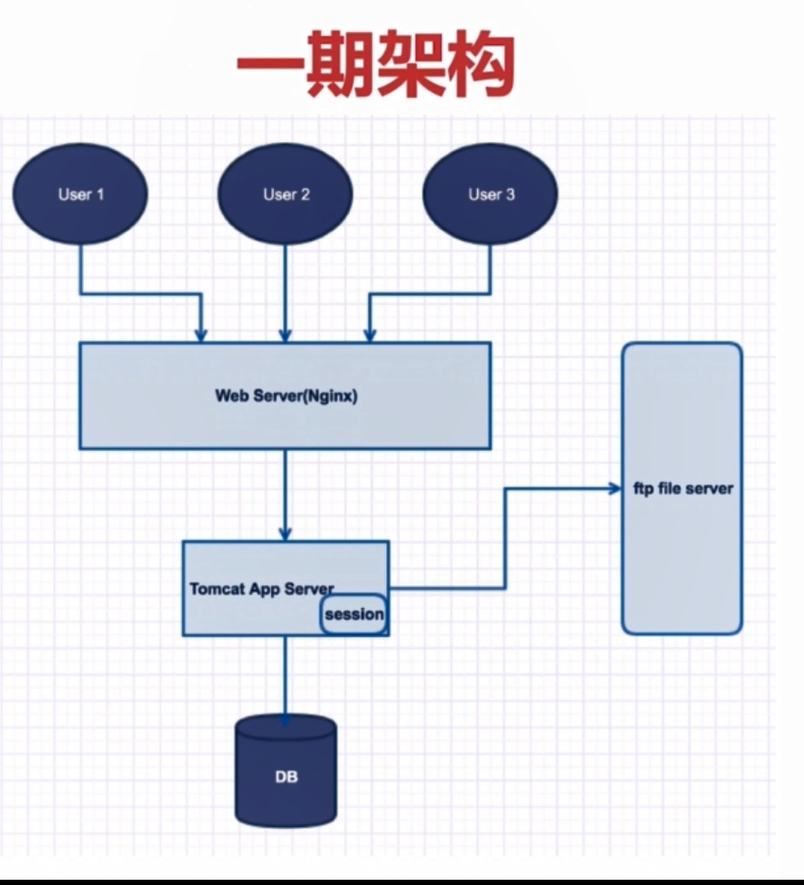
\includegraphics[width=0.7\linewidth]{figures/happymmallOne.png}
	\caption{happymmallOne}
	\label{fig:happymmallOne}
\end{figure}

(\textbf{二期架构})

软件架构: Spring + SpringMVC + Mybatis + Nginx + Tomcat + Redis + Jedis + Lombok + Jackson + Guava Cache

使用横向扩展, 将session存储到redis中. 使用maven进行环境隔离, 分为 local dev 和prod 环境, lombok进行代码整洁性优化. 使用nginx进行负载均衡, 简单来说就是将请求分发到不同的tomcat中, 以权重的方式. redis使用一致性hash算法进行缓存分片部署.封装了异常处理防止服务端关键信息泄露. 分布式锁进行了优化防止死锁.




一致性hash算法介绍:
简单来说生成多个虚拟节点, 以 0 ~ $2^31-1$ 的范围进行部署, 然后看顺时针映射到哪一个redis容器中.


Jackson: 主要通过objectMapper对象来实现json转string操作和string转json操作. 主要用在存储redis中的sessionid所存储的对象. 使用hash方式存储

slf4j+lockback: 进行日志管理 lockback 读取配置文件logback.xml进行解析

md5: 进行密码的加盐处理

Lombok: 用来简化代码的编写. 使用代码更加清晰

<mvc:interceptor> + handlerinterceptor: 使用拦截器来进行. 防止没有需要登陆的操作被使用. 如果是登陆操作使用单独的逻辑 当然也可以使用相关的配置

用户模块, 登陆注册, 忘记密码, 其中忘记密码要重置的时候携带的token也是存放在redis中的

商品模块, 可以查看商品的详细信息, 使用了mybatis 的 pagehelper 分页器插件, 使用拦截器对sql进行limit处理


另一个我想介绍的是购物车模块.
购物车模块在展示购物车中选中的物品的时候, 使用DigDecimal类来进行数值的统计, 防止出现用为java, double有效位数导致的金额错误. 其中 bigDecimal类 我们需要使用String类型的构造函数, 因为使用double类型的构造函数还是会出现精度问题.

\begin{figure}
	\centering
	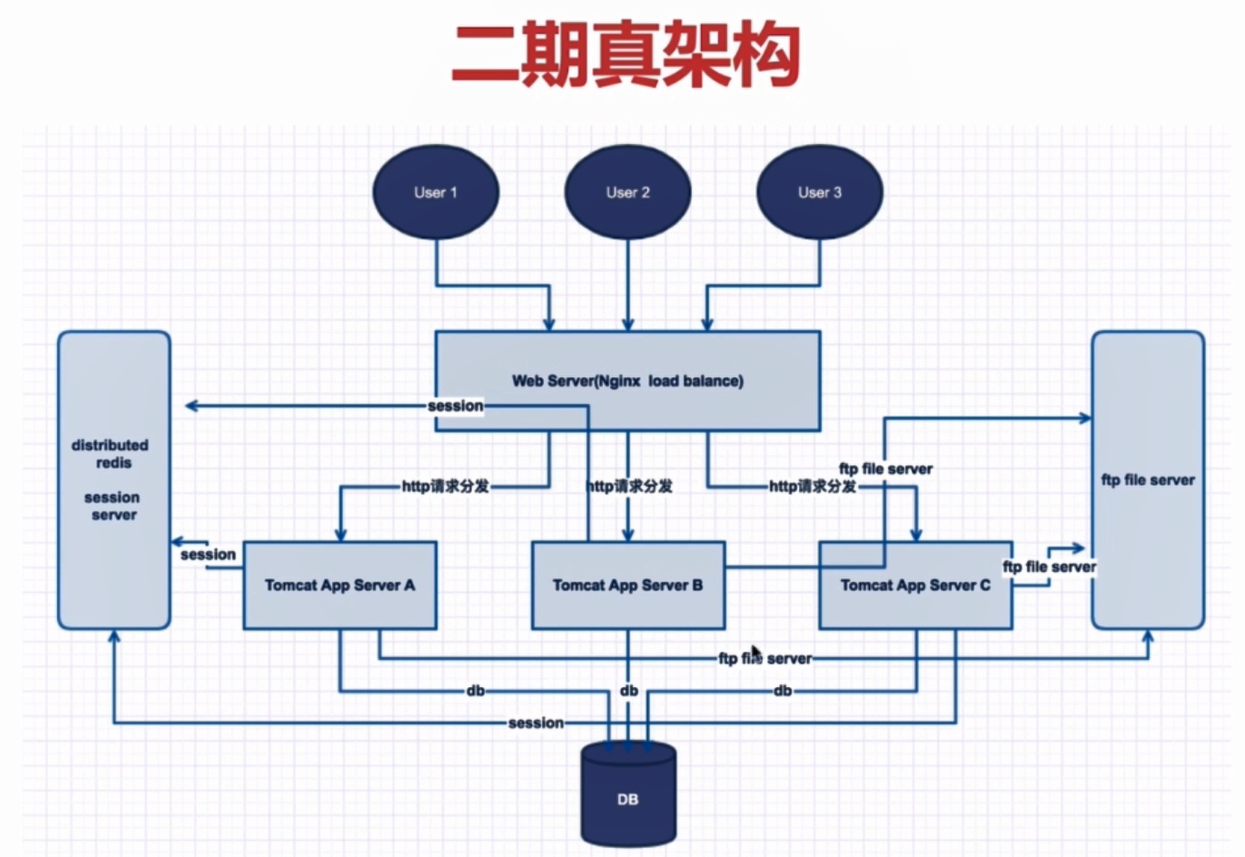
\includegraphics[width=0.7\linewidth]{figures/happymmallTwo.png}
	\caption{happymmallTwo}
	\label{fig:happymmallTwo}
\end{figure}

\begin{figure}
	\centering
	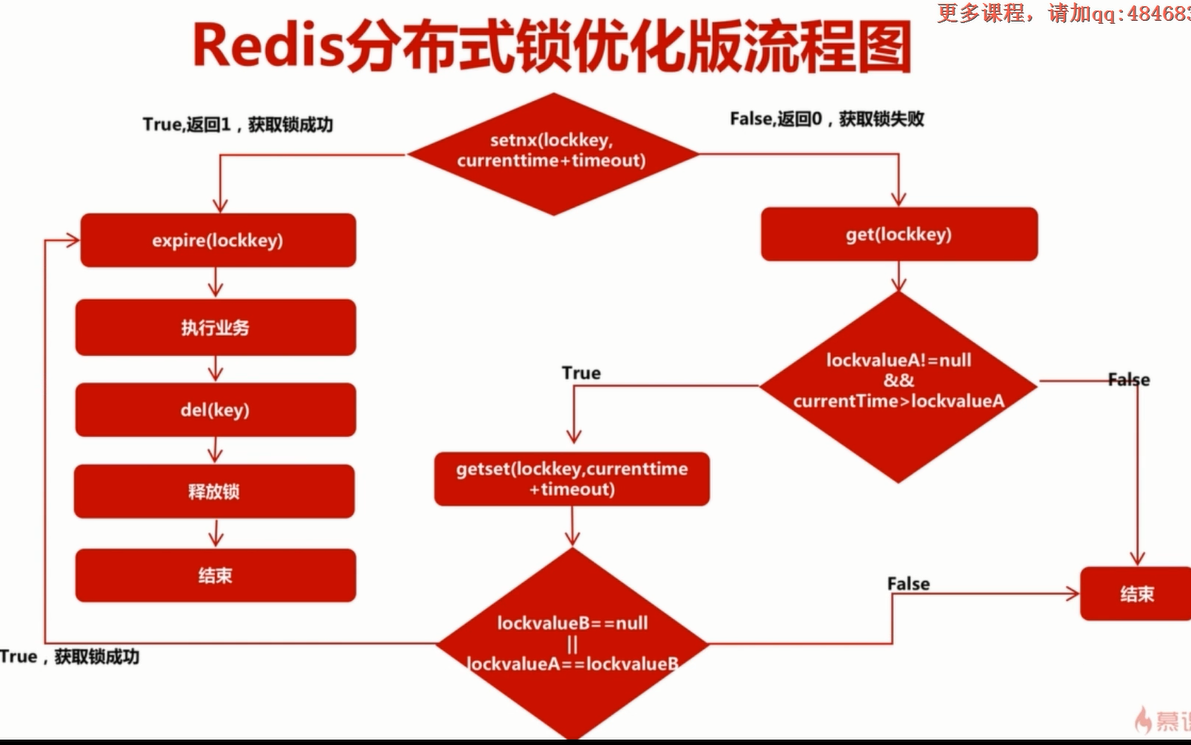
\includegraphics[width=0.7\linewidth]{figures/redislockdistribution.png}
	\caption{redislockdistribution}
	\label{fig:redislockdistribution}
\end{figure}

\begin{figure}
	\centering
	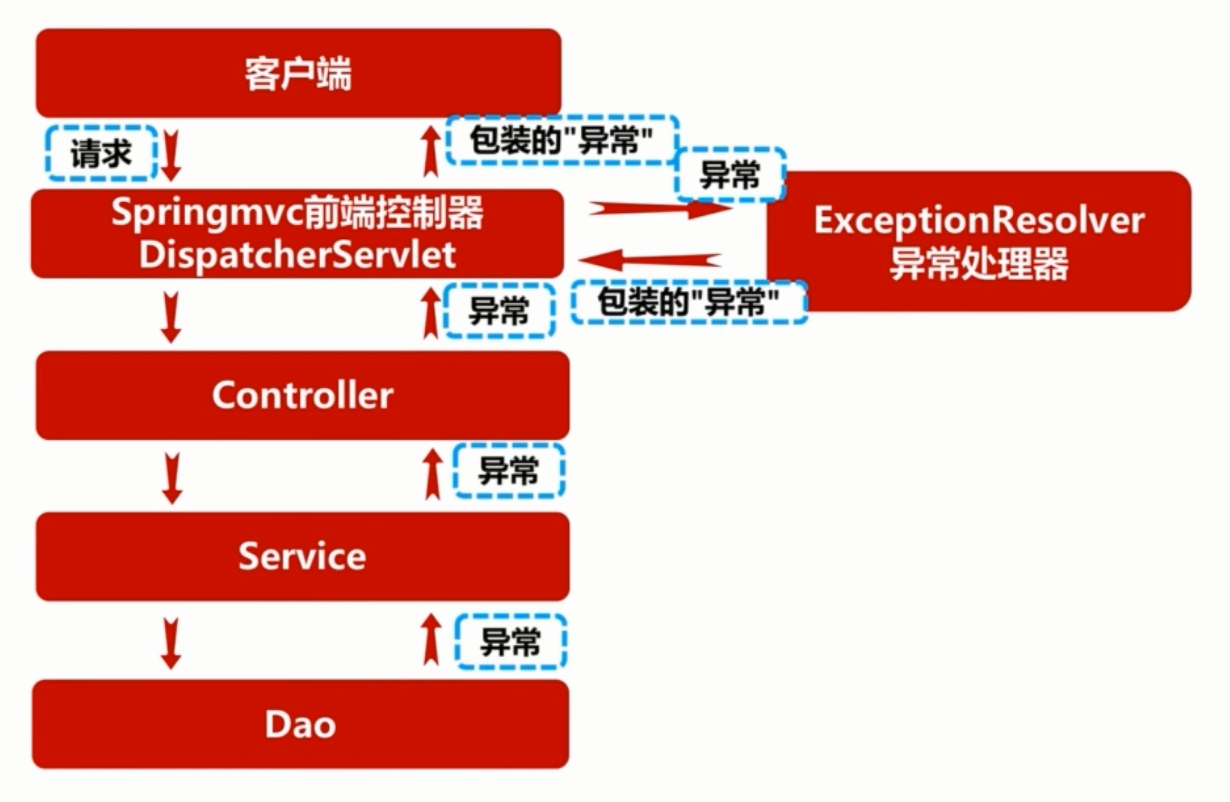
\includegraphics[width=0.7\linewidth]{figures/happymmallexception.png}
	\caption{happymmallexception}
	\label{fig:happymmallexception}
\end{figure}

\subsubsection{秒杀项目介绍}

mysql + reids + springboot + rockmq + nginx + @Transactional

1. 为什么要讲商品的库存表item\_stock与商品表分开?

库存操作非常耗时、性能,在商品交易过程中库存减,如果合并到item表中,每次会对对应行加行锁。如果分开库存表,虽然每次减库存过程还是会加行锁,但是可以将这张表拆到另一个数据库当中,分库分表,做效果的优化


@CrossOrigin(origins = {"*"},allowCredentials = "true")

我们的ajax看到这两个头部就认定对应的域名接收任何来自或不来自于本域的请求, 简单来说,就是请求地址和域名请求都可以

2. tomcat 参数优化

增加线程数数量, 最大工作线程数量增加到了200

keepAliveTimeOut:  设置30秒内没有请求则服务端自动断开keepalive链接

maxKeepAliveRequests: 当客户端发送超过10000个请求则自动断开keepalive链接

一定程度上减少了TCP三次握手的时间损耗.

3. 水平扩展

将前端静态资源直接放在nginx里面的html目录中. 基于token的会话管理, 前端存储到localStorage. 后端存储到redis


4. 多级缓存

使用了三级缓存, 第一级使用了guawacache存储了商品的信息, 第二级 redis 第三季 数据库
使用序列化方式进行存储. 商品列表 可以达到Average time 150ms,对应的Tps:2000/s,对应的redis几乎没有任何压力,
缓存机制从redis缓存加载到了jvm缓存之后,减少了多段的网络开销,并且完成了对应的内存访问输出结果,性能提升明显,但是数据更新之后缓存失效,还有JVM容量大小的限制;

5. 数据库库存 放入redis

会产生数据不一致的现象.

(1)活动发布同步库存进缓存

(2)下单交易减缓存库存

(3)异步消息扣减数据库内存

RocketMQ主要有 Producer端,负责向Broker发送消息;Consumer端,多个consumer组成一个ConsumerGroup,每个消息会有一个Group里的consumer来消费;Broker由topic和MessageQueue组成,消息隶属于某个topic,一个topic可能由一个或多个topic管理


Producer连接NameServer发现broker1,会向topicA为主题的broker1投递消息,采用负载轮询向queue投递;

Consumer抓取负责的topicA,与queue建立长连接,当有消息时,唤醒,拉取对应的message,没有消息就等待,这种方式叫做长轮询

我们的解决方法就是异步消息的发送要在整个事务提交成功后再发送

6. 秒杀令牌

活动开始生成令牌

7. 设置秒杀大闸

就是一次释放的令牌大约是库存的5倍, + 验证码防止黄牛操作

8. 限流

使用令牌桶算法则是一个存放固定容量令牌的桶,按照固定速率往桶里添加令牌。桶中存放的令牌数有最大上限,超出之后就被丢弃或者拒绝。当流量或者网络请求到达时,每个请求都要获取一个令牌,如果能够获取到,则直接处理,并且令牌桶删除一个令牌。如果获取不同,该请求就要被限流,要么直接丢弃,要么在缓冲区等待。

Guava RateLimiter


使用 RateLimiter的静态方法创建一个限流器,设置每秒放置的令牌数为5个。返回的RateLimiter对象可以保证1秒内不会给超过5个令牌,并且以固定速率进行放置,达到平滑输出的效果。

9. 数据流

下单->流水库存->真正库存


10. 活动的开启与关闭, 通过一个内部的接口实现.

\subsubsection{英文项目介绍}

It’s difficult to construct hexahedral meshes currently, this paper presents an interactive construction method of complex hexahedral mesh model based on volumetric subdivision. The user firstly needs to in-teractively construct the model skeleton, by placing cubes at the nodes of the skeleton structure, and per-forming interactive operations such as rotation, translation, and scaling of the node cubes. Then, through the connection between the nodes and the topological split operation, the initial control mesh can be con-structed. Further, interpolatory Catmull-Clark volumetric subdivision method is used to generate hexahe-dral meshes with different resolutions; finally, the padding operation is used to eliminate the degraded ele-ments at the boundary and improve the quality of the hexahedral mesh elements to obtain the final hexahe-dral mesh. The results of numerical example show that the method can easily and efficiently generate hex-ahedral meshes interactively, and eliminat the intermediate steps of generating volume meshes from surface meshes. It has some practical applications in finite element analysis, isogeometric analysis and geometric modeling in animation.

\begin{figure}
	\centering
	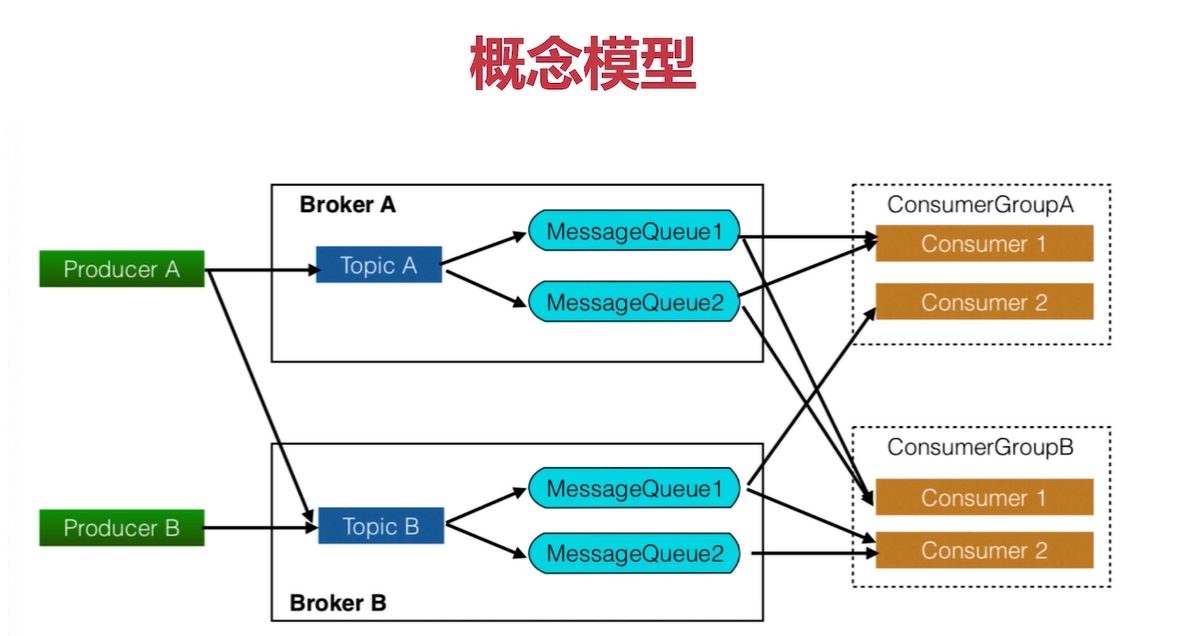
\includegraphics[width=0.7\linewidth]{figures/rockmq.png}
	\caption{rockmq}
	\label{fig:rockmq}
\end{figure}
